\documentclass[../../main.tex]{subfiles}

\graphicspath{{../../image/}{../../figure/}}

\begin{document}

\section{Langevin 采样}\label{section:ch14-langevin采样}

Metropolis-Hastings 算法通过使用提议分布创建候选样本的 Markov 链，并使用\eqref{align:ch14-mh接受概率}所示的准则接受或拒绝它们，从而从概率分布中抽取样本。这可能相对低效，因为提议分布通常是一个简单且固定的分布，它可以在数据空间的任何方向上生成更新，从而导致随机游走的行为。

我们已经看到，在训练神经网络时，利用关于模型可学习参数的对数似然梯度来最大化似然函数是极其有利的。类似地，我们可以引入利用关于数据向量的概率密度梯度的 Markov 链采样算法，以便优先向概率较大的区域移动。这种技术称为 Hamiltonian Monte Carlo 采样，也称混合 Monte Carlo（hybrid Monte Carlo）采样。该采样方法使用了 Metropolis 接受准则（Duane et al., 1987; Bishop, 2006）。在这里，我们研究一种在深度学习中使用广泛的新的采样方法——Langevin 采样。尽管它避免了使用 Metropolis 接受准则，但我们必须仔细设计算法，以确保产生的结果样本是无偏的。在基于能量函数的机器学习模型中，Langevin 采样发挥了至关重要的作用。

\subsection{基于能量的模型}\label{subsection:ch14-基于能量的模型}

许多生成式模型可以表示为条件概率分布 $p(\bm{x}\mid\bm{w})$，其中 $\bm{x}$ 是数据向量，$\bm{w}$ 代表可学习参数的向量。这样的模型可以通过最大化相对于训练集定义的对应似然函数来进行训练。然而，为了表示一个有效的概率分布，模型必须满足如下要求：
\begin{align}
\int p(\bm{x}\mid\bm{w})\,p(\bm{x})\,\mathrm{d}\bm{x}=1.
\label{align:ch14-归一化}
\end{align}

\begin{remark}（重构新增）\textbf{原文问题说明。}原书\eqref{align:ch14-归一化}印作 $\int p(\bm{x}\mid\bm{w})p(\bm{x})\mathrm{d}\bm{x}=1$，但归一化要求针对的是条件密度本身，正确形式应为
\begin{align*}
\int p(\bm{x}\mid\bm{w})\,\mathrm{d}\bm{x}=1.
\end{align*}
上式多出的因子 $p(\bm{x})$ 会使积分依赖于 $\bm{x}$ 的先验分布，从而无法对一切 $\bm{w}$ 恒等于 $1$，与「模型是有效概率分布」这一要求不符。本译本保留原式以忠实于原书，但本章此后的一切推导（特别是\eqref{align:ch14-ebm}与\eqref{align:ch14-partition}）均按修正后的归一化形式进行。这一处属于排版或翻译层面的笔误，不影响后续数学内容。
\end{remark}

这样的归一化要求大大限制了适用模型的形式。在不考虑归一化约束的情况下，我们可以考虑一个更广泛的模型类别，称为基于能量的模型（LeCun et al., 2006）。假设我们有一个称为能量函数的函数 $E(\bm{x},\bm{w})$，它是其参数的实值函数，但没有其他约束。指数 $\exp\{-E(\bm{x},\bm{w})\}$ 是一个非负数，因此可以看作未归一化的 $\bm{x}$ 上的概率分布。这里在指数中引入负号只是一个惯例，它意味着能量的较高值对应于概率的较低值。然后我们可以使用下式定义一个归一化的分布（见\cref{exercise:ch14-16}）：
\begin{align}
p(\bm{x}\mid\bm{w})=\frac{1}{Z(\bm{w})}\exp\{-E(\bm{x},\bm{w})\},
\label{align:ch14-ebm}
\end{align}
其中归一化常数 $Z(\bm{w})$ 称为配分函数（partition function），它由下式定义：
\begin{align}
Z(\bm{w})=\int\exp\{-E(\bm{x},\bm{w})\}\,\mathrm{d}\bm{x}.
\label{align:ch14-partition}
\end{align}

\begin{definition}[基于能量的模型]\label{definition:ch14-基于能量模型}
设 $E(\bm{x},\bm{w})$ 是数据向量 $\bm{x}$ 与参数 $\bm{w}$ 的实值函数，称为能量函数，且
\begin{align*}
0<Z(\bm{w})=\int\exp\{-E(\bm{x},\bm{w})\}\,\mathrm{d}\bm{x}<\infty.
\end{align*}
则由\eqref{align:ch14-ebm}定义的分布族 $\left\{p(\bm{x}\mid\bm{w})\right\}$ 称为基于能量的模型（energy-based model，EBM），$Z(\bm{w})$ 称为配分函数（partition function）。
\end{definition}

% SUPPLEMENT: parent=definition:ch14-基于能量模型; kind=motivation; location=紧随其后的 remark（重构新增）
\begin{remark}（重构新增）基于能量的模型把「概率建模」化为「设计一个打分函数」：能量 $E$ 可以任意选取（例如用深度神经网络实现），只要指数可积，\eqref{align:ch14-ebm}就自动给出一个合法的概率分布。负号约定使「低能量＝高概率」，从而训练可以理解为「给数据点分配低能量、给模型样本分配高能量」。定义中 $0<Z(\bm{w})<\infty$ 的条件不可省：$Z=0$ 时密度无定义，$Z=\infty$ 时密度不可归一化，此时 $p$ 只是「未归一化的分数函数」而非概率分布。配分函数是全部困难的来源——它是对整个 $\bm{x}$ 空间（或全部离散状态）的积分，高维时无法精确计算，\cref{subsection:ch14-最大化似然}与\cref{subsection:ch14-langevin动力学}的全部技巧都是为了绕开它。最后，任何归一化的概率模型都可以写成\eqref{align:ch14-ebm}的形式（取 $E=-\ln p$），因此 EBM 是一个包含极广的框架，其代价是 $Z$ 通常不可解。
\end{remark}

\begin{definition}[配分函数]\label{definition:ch14-配分函数}
对能量函数 $E(\bm{x},\bm{w})$，称
\begin{align*}
Z(\bm{w})=\int\exp\{-E(\bm{x},\bm{w})\}\,\mathrm{d}\bm{x}
\end{align*}
为配分函数；离散变量情形下积分替换为求和 $Z(\bm{w})=\sum_{\bm{x}}\exp\{-E(\bm{x},\bm{w})\}$。
\end{definition}

% SUPPLEMENT: parent=definition:ch14-配分函数; kind=motivation; location=紧随其后的 remark（重构新增）
\begin{remark}（重构新增）配分函数之名来自统计物理：$Z$ 是 Boltzmann 因子 $e^{-E}$ 对所有状态的总和，$\ln Z$ 对应自由能。它在数学上只起归一化作用，却出现在对数似然的梯度中（见\eqref{align:ch14-grad-nll}），因此无法像对待普通常数那样忽略。计算 $Z$ 的困难有两个来源：其一是积分区域是高维的，网格法的代价随维数指数增长；其二是 $E$ 通常由神经网络给出，没有解析结构。这两种困难正是本章后文用 Markov 链 Monte Carlo 与 Langevin 动力学近似 $Z$ 的梯度（而非 $Z$ 本身）的动机。注意 $Z$ 只依赖 $\bm{w}$ 而不依赖 $\bm{x}$，这一事实在\eqref{align:ch14-grad-expected}中被用来把 $-\nabla_{\bm{w}}\ln Z$ 移出关于 $\bm{x}$ 的期望。
\end{remark}

能量函数通常使用深度神经网络进行建模，输入向量为 $\bm{x}$，标量输出为 $E(\bm{x},\bm{w})$，其中 $\bm{w}$ 代表网络中权重和偏置的集合。

注意配分函数依赖于 $\bm{w}$，这给训练带来了一些问题。例如，一组独立同分布数据 $\mathcal{D}=\left\{\bm{x}_{1},\cdots,\bm{x}_{N}\right\}$ 的对数似然函数具有以下形式：
\begin{align}
\ln p(\mathcal{D}\mid\bm{w})=-\sum_{n=1}^{N}E\!\left(\bm{x}_{n},\bm{w}\right)-N\ln Z(\bm{w}).
\label{align:ch14-ebm-nll}
\end{align}

要计算 $\ln p(\mathcal{D}\mid\bm{w})$ 关于 $\bm{w}$ 的梯度，我们需要知道 $Z(\bm{w})$ 的形式。然而，对于具有许多选择的能量函数 $E(\bm{x},\bm{w})$，计算配分函数\eqref{align:ch14-partition}是不切实际的，因为这需要对整个 $\bm{x}$ 空间进行积分（或对离散变量求和）。「基于能量的模型」指的就是这种积分难以处理的模型。然而请注意，概率模型可以视为基于能量的模型的特例，因此本书讨论的许多模型可以视为基于能量的模型。基于能量的模型的最大优势是，它们在不需要归一化的情况下具有灵活性。相应的缺点是，由于归一化常数未知，它们可能更难以训练。

\subsection{最大化似然}\label{subsection:ch14-最大化似然}

我们已经开发了各种近似方法来训练基于能量的模型，而无须计算配分函数（Song and Kingma, 2021）。本小节探讨基于 Markov 链 Monte Carlo 采样的技术。另一种方法称为分数匹配，我们将在扩散模型的背景下进行讨论（见\cref{chapter:ch20-扩散模型}）。

我们已经看到，对于基于能量的模型，由于存在未知的配分函数 $Z(\bm{w})$，似然函数不能显式求值。然而，我们可以利用 Monte Carlo 采样方法，来计算对数似然函数关于模型参数的梯度。一旦以任何方式训练了基于能量的模型，就可以使用采样方法从模型中抽取样本了，比如使用 Monte Carlo 采样方法。

使用\eqref{align:ch14-ebm}，对于一个基于能量的模型，对数似然函数关于模型参数的梯度可以写成以下形式：
\begin{align}
\nabla_{\bm{w}}\ln p(\bm{x}\mid\bm{w})=-\nabla_{\bm{w}}E(\bm{x},\bm{w})-\nabla_{\bm{w}}\ln Z(\bm{w}).
\label{align:ch14-grad-nll}
\end{align}

\begin{proposition}[对数似然的梯度]\label{proposition:ch14-对数似然梯度}
设 $p(\bm{x}\mid\bm{w})$ 由\eqref{align:ch14-ebm}给出，$E$ 关于 $\bm{w}$ 可微，且可在积分号下求导。则\eqref{align:ch14-grad-nll}成立。
\end{proposition}

\begin{proof}
对\eqref{align:ch14-ebm}取对数得 $\ln p(\bm{x}\mid\bm{w})=-E(\bm{x},\bm{w})-\ln Z(\bm{w})$，对 $\bm{w}$ 求梯度即得\eqref{align:ch14-grad-nll}。
\end{proof}

% SUPPLEMENT: parent=proposition:ch14-对数似然梯度; kind=motivation; location=紧随其后的 remark（重构新增）
\begin{remark}（重构新增）这个恒等式本身只是「对数把乘积变和」的结果，它的意义在于把梯度分成两项：第一项 $-\nabla_{\bm{w}}E(\bm{x},\bm{w})$ 可以直接由自动微分算出；第二项 $-\nabla_{\bm{w}}\ln Z(\bm{w})$ 涉及配分函数，需要借助采样来估计（见\eqref{align:ch14-partition-grad}）。条件「可在积分号下求导」保证了 $\nabla_{\bm{w}}Z=\int\nabla_{\bm{w}}e^{-E}\,\mathrm{d}\bm{x}$，在 $E$ 关于 $\bm{w}$ 局部 Lipschitz、$e^{-E}$ 可积且有可积控制函数时成立，这是后续一切推导的前提。若该条件失效（例如 $E$ 的梯度无界），梯度与积分不可交换，公式需要重新论证。
\end{remark}

这是针对单个数据点 $\bm{x}$ 的似然函数，但实际上我们希望最大化训练数据集上的似然函数，该数据集是从某个未知分布 $p_{D}(\bm{x})$ 中抽样得到的。如果我们假设数据点是独立同分布的，那么我们可以考虑与 $p_{D}(\bm{x})$ 相关的似然对数期望的梯度，其由下式给出：
\begin{align}
\mathbb{E}_{\bm{x}\sim p_{D}}\left[\nabla_{\bm{w}}\ln p(\bm{x}\mid\bm{w})\right]=-\mathbb{E}_{\bm{x}\sim p_{D}}\left[\nabla_{\bm{w}}E(\bm{x},\bm{w})\right]-\nabla_{\bm{w}}\ln Z(\bm{w}).
\label{align:ch14-grad-expected}
\end{align}
这里我们利用了 $-\nabla_{\bm{w}}\ln Z(\bm{w})$ 不依赖于 $\bm{x}$ 的性质，因而可以把它移到期望之外。假设配分函数 $Z(\bm{w})$ 是未知的，但我们可以利用\eqref{align:ch14-partition}并重组得到
\begin{align}
-\nabla_{\bm{w}}\ln Z(\bm{w})=\int\left\{\nabla_{\bm{w}}E(\bm{x},\bm{w})\right\}p(\bm{x}\mid\bm{w})\,\mathrm{d}\bm{x}.
\label{align:ch14-partition-grad}
\end{align}

\begin{proposition}[配分函数对数的梯度]\label{proposition:ch14-配分函数梯度}
在\cref{proposition:ch14-对数似然梯度}的条件下，\eqref{align:ch14-partition-grad}成立，即
\begin{align*}
-\nabla_{\bm{w}}\ln Z(\bm{w})=\mathbb{E}_{p(\bm{x}\mid\bm{w})}\left[\nabla_{\bm{w}}E(\bm{x},\bm{w})\right].
\end{align*}
\end{proposition}

\begin{proof}
由 $Z(\bm{w})=\int e^{-E(\bm{x},\bm{w})}\mathrm{d}\bm{x}$ 及积分号下求导，
\begin{align*}
\nabla_{\bm{w}}Z(\bm{w})=\int\nabla_{\bm{w}}e^{-E(\bm{x},\bm{w})}\,\mathrm{d}\bm{x}=-\int\left\{\nabla_{\bm{w}}E(\bm{x},\bm{w})\right\}e^{-E(\bm{x},\bm{w})}\,\mathrm{d}\bm{x}.
\end{align*}
两边除以 $Z(\bm{w})$ 并用\eqref{align:ch14-ebm}：
\begin{align*}
\nabla_{\bm{w}}\ln Z(\bm{w})=\frac{\nabla_{\bm{w}}Z(\bm{w})}{Z(\bm{w})}=-\int\left\{\nabla_{\bm{w}}E(\bm{x},\bm{w})\right\}\frac{e^{-E(\bm{x},\bm{w})}}{Z(\bm{w})}\,\mathrm{d}\bm{x}=-\int\left\{\nabla_{\bm{w}}E(\bm{x},\bm{w})\right\}p(\bm{x}\mid\bm{w})\,\mathrm{d}\bm{x},
\end{align*}
移项即得\eqref{align:ch14-partition-grad}。
\end{proof}

% SUPPLEMENT: parent=proposition:ch14-配分函数梯度; kind=motivation; location=紧随其后的 remark（重构新增）
\begin{remark}（重构新增）这个结果通常称为「对数配分函数的梯度等于能量的负梯度在模型分布下的期望」，它是全部对比散度方法的核心恒等式：右侧只涉及模型分布 $p(\bm{x}\mid\bm{w})$ 下的期望，而不涉及 $Z$ 本身，因此只要能从模型采样就能估计。证明中「积分号下求导」与「除以 $Z$」两步分别需要\cref{proposition:ch14-对数似然梯度}的条件与 $Z>0$；$Z=0$ 时对数无定义，$Z=\infty$ 时比值无意义，这正是\cref{definition:ch14-基于能量模型}要求 $0<Z<\infty$ 的原因。注意该式对任意 $\bm{w}$ 都成立，并不要求 $\bm{w}$ 已是最优参数。
\end{remark}

\eqref{align:ch14-partition-grad}右侧的部分对应于模型分布 $p(\bm{x}\mid\bm{w})$ 的期望，它由下式给出（见\cref{exercise:ch14-18}）：
\begin{align}
\int\left\{\nabla_{\bm{w}}E(\bm{x},\bm{w})\right\}p(\bm{x}\mid\bm{w})\,\mathrm{d}\bm{x}=\mathbb{E}_{\bm{x}\sim p_{M}}\left[\nabla_{\bm{w}}E(\bm{x},\bm{w})\right],
\label{align:ch14-model-expectation}
\end{align}
其中 $p_{M}(\bm{x})$ 表示模型分布 $p(\bm{x}\mid\bm{w})$。结合\eqref{align:ch14-grad-expected}～\eqref{align:ch14-model-expectation}，我们得到
\begin{align}
\nabla_{\bm{w}}\mathbb{E}_{\bm{x}\sim p_{D}}\left[\ln p(\bm{x}\mid\bm{w})\right]=-\mathbb{E}_{\bm{x}\sim p_{D}}\left[\nabla_{\bm{w}}E(\bm{x},\bm{w})\right]+\mathbb{E}_{\bm{x}\sim p_{M}(\bm{x})}\left[\nabla_{\bm{w}}E(\bm{x},\bm{w})\right].
\label{align:ch14-对比散度梯度}
\end{align}

\begin{theorem}[对比散度梯度]\label{theorem:ch14-对比散度梯度}
在\cref{proposition:ch14-配分函数梯度}的条件下，记 $p_{M}=p(\cdot\mid\bm{w})$，则对数似然期望的梯度由\eqref{align:ch14-对比散度梯度}给出。
\end{theorem}

\begin{proof}
把\eqref{align:ch14-partition-grad}代入\eqref{align:ch14-grad-expected}，并用\eqref{align:ch14-model-expectation}把积分写成关于 $p_{M}$ 的期望：
\begin{align*}
\nabla_{\bm{w}}\mathbb{E}_{p_{D}}\left[\ln p(\bm{x}\mid\bm{w})\right]&=-\mathbb{E}_{p_{D}}\left[\nabla_{\bm{w}}E(\bm{x},\bm{w})\right]-\nabla_{\bm{w}}\ln Z(\bm{w})\\
&=-\mathbb{E}_{p_{D}}\left[\nabla_{\bm{w}}E(\bm{x},\bm{w})\right]+\mathbb{E}_{p_{M}}\left[\nabla_{\bm{w}}E(\bm{x},\bm{w})\right],
\end{align*}
即\eqref{align:ch14-对比散度梯度}。
\end{proof}

% SUPPLEMENT: parent=theorem:ch14-对比散度梯度; kind=motivation; location=紧随其后的 remark（重构新增）
\begin{remark}（重构新增）\eqref{align:ch14-对比散度梯度}把梯度写成两个期望之差：一项在数据分布下、一项在模型分布下，故称为「正相」与「负相」，其差也常称为对比散度。两相的作用相反：正相（第一项，带负号）降低数据点处的能量，从而提高数据点的概率；负相（第二项，带正号）提高模型样本处的能量，从而压低模型自身产生的样本的概率。当且仅当 $p_{M}=p_{D}$ 时两相相等、梯度为零，因此该式的驻点条件正是「模型分布与数据分布匹配」。这一形式要求能从 $p_{M}$ 采样——而 $p_{M}$ 恰恰含有未知的 $Z$，于是问题转化为「如何从 EBM 采样」，这正是\cref{subsection:ch14-langevin动力学}的主题。注意\eqref{align:ch14-对比散度梯度}是\emph{期望}的梯度，与单个数据点的梯度\eqref{align:ch14-grad-nll}不同，实际训练用 mini-batch 估计前者。
\end{remark}

\begin{figure}[htbp]
\centering
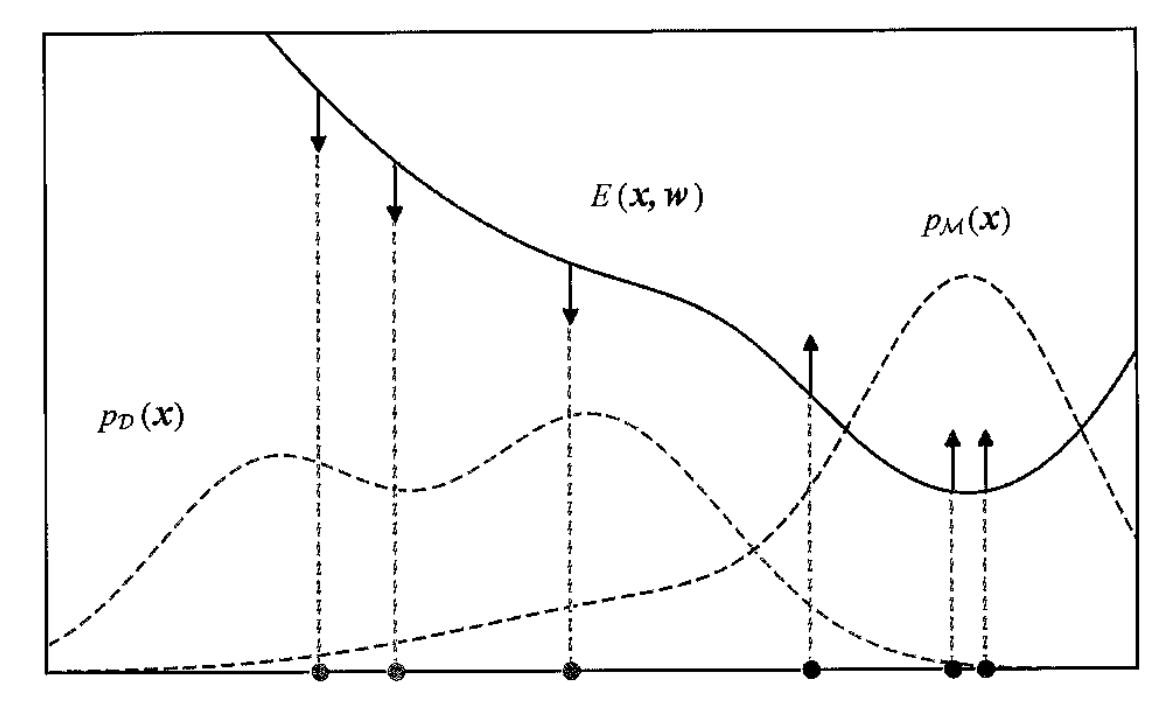
\includegraphics[width=0.72\textwidth]{ch14-fig14.13-energy.png}
\caption{通过最大化似然对基于能量的模型进行训练的示意图，其中显示了能量函数 $E(\bm{x},\bm{w})$（绿色）及相关的模型分布 $p_{M}(\bm{x})$ 和真实数据分布 $p_{D}(\bm{x})$。利用\eqref{align:ch14-对比散度梯度}增加期望的对数似然，会在与模型样本（用蓝点表示）对应的点处推高能量函数，并在与数据集样本（用红点表示）对应的点处拉低能量函数}
\label{figure:ch14-能量模型训练}
\end{figure}

\cref{figure:ch14-能量模型训练}对这个结果做了说明，详细解释如下。我们的目标是找到参数 $\bm{w}$ 的值，让似然函数的值最大化。为此，我们朝梯度 $\nabla_{\bm{w}}\ln p(\bm{x}\mid\bm{w})$ 的方向对 $\bm{w}$ 进行了微小调整。从\eqref{align:ch14-对比散度梯度}中可以看出，这个梯度的期望值可以分解为两部分，且这两部分符号相反。\eqref{align:ch14-对比散度梯度}右侧第一项的作用是减小 $E(\bm{x},\bm{w})$，因而会增大模型定义的数据点 $\bm{x}$ 的概率密度，这里的 $\bm{x}$ 是从 $p_{D}(\bm{x})$ 中抽取的。\eqref{align:ch14-对比散度梯度}右侧第二项的作用则是增大 $E(\bm{x},\bm{w})$，从而降低由模型定义的来自模型本身的数据点的概率密度。在模型密度超过训练数据密度的区域，净效果将是增加能量，因此降低了概率密度。相反，在训练数据密度超过模型密度的区域，净效果将是降低能量，因此增大了概率密度。正如我们所希望的那样，这两项一起将概率密度从训练数据密度低的区域移向了训练数据密度高的区域。当模型分布与数据分布相匹配时，这两项将在幅度上相等，此时\eqref{align:ch14-对比散度梯度}左侧的梯度就等于零。

\subsection{Langevin 动力学}\label{subsection:ch14-langevin动力学}

当把\eqref{align:ch14-对比散度梯度}作为一种实际的训练方法应用时，我们需要近似计算\eqref{align:ch14-对比散度梯度}右侧的两项。对于任何给定的 $\bm{x}$ 值，我们可以使用自动微分来评估 $\nabla_{\bm{w}}E(\bm{x},\bm{w})$。对于\eqref{align:ch14-对比散度梯度}中的第一项，我们可以使用训练集来估计关于 $\bm{x}$ 的期望：
\begin{align}
\mathbb{E}_{\bm{x}\sim p_{D}}\left[\nabla_{\bm{w}}E(\bm{x},\bm{w})\right]\approx\frac{1}{N}\sum_{n=1}^{N}\nabla_{\bm{w}}E\!\left(\bm{x}_{n},\bm{w}\right).
\label{align:ch14-数据期望}
\end{align}

\eqref{align:ch14-对比散度梯度}中的第二项更具挑战性，因为我们需要从能量函数定义的模型分布中抽取样本，而相应的配分函数难以处理。这可以使用 Markov 链 Monte Carlo 采样来完成。另一种受欢迎的采样方法称为随机梯度 Langevin 动力学，简称 Langevin 采样（Parisi, 1981; Welling and Teh, 2011）。这一项仅通过得分函数（score function）依赖于分布 $p(\bm{x}\mid\bm{w})$，得分函数定义为对数似然函数关于数据向量 $\bm{x}$ 的梯度，并由下式给出：
\begin{align}
\bm{s}(\bm{x},\bm{w})=\nabla_{\bm{x}}\ln p(\bm{x}\mid\bm{w}).
\label{align:ch14-得分函数}
\end{align}

\begin{definition}[得分函数]\label{definition:ch14-得分函数}
设 $p(\bm{x}\mid\bm{w})$ 关于 $\bm{x}$ 可微且为正，称
\begin{align*}
\bm{s}(\bm{x},\bm{w})=\nabla_{\bm{x}}\ln p(\bm{x}\mid\bm{w})
\end{align*}
为分布 $p(\cdot\mid\bm{w})$ 的得分函数（score function）。
\end{definition}

% SUPPLEMENT: parent=definition:ch14-得分函数; kind=motivation; location=紧随其后的 remark（重构新增）
\begin{remark}（重构新增）得分函数是「对数密度关于\emph{数据}的梯度」，与通常的「关于参数 $\bm{w}$ 的梯度」完全不同：前者指向「往哪个方向移动 $\bm{x}$ 能使密度增大」，后者指向「怎样调整参数能使似然增大」。这一区分是理解本节的钥匙：训练需要后者，而从模型采样需要前者。得分函数不依赖归一化常数，因为 $\nabla_{\bm{x}}\ln Z(\bm{w})=0$（$Z$ 与 $\bm{x}$ 无关），这使得它成为绕开配分函数的天然工具——它正是扩散模型中分数匹配方法的出发点。定义要求 $p>0$ 且可微，否则对数梯度无定义；在支撑集边界附近得分函数可能发散，这是数值实现时需要裁剪的原因之一。
\end{remark}

值得强调的是，这是针对数据点 $\bm{x}$ 的梯度，而非通常意义上针对可学习参数 $\bm{w}$ 的梯度。将\eqref{align:ch14-ebm}代入\eqref{align:ch14-得分函数}，我们可以得到
\begin{align}
\bm{s}(\bm{x},\bm{w})=-\nabla_{\bm{x}}E(\bm{x},\bm{w}).
\label{align:ch14-得分能量}
\end{align}
可以看到，配分函数不再出现，因为它与 $\bm{x}$ 无关。

\begin{proposition}[得分函数与能量函数]\label{proposition:ch14-得分与能量}
设 $p(\bm{x}\mid\bm{w})$ 由\eqref{align:ch14-ebm}给出，$E$ 关于 $\bm{x}$ 可微。则\eqref{align:ch14-得分能量}成立。
\end{proposition}

\begin{proof}
对 $\ln p(\bm{x}\mid\bm{w})=-E(\bm{x},\bm{w})-\ln Z(\bm{w})$ 关于 $\bm{x}$ 求梯度。由于 $Z(\bm{w})$ 与 $\bm{x}$ 无关，$\nabla_{\bm{x}}\ln Z(\bm{w})=\bm{0}$，故 $\nabla_{\bm{x}}\ln p(\bm{x}\mid\bm{w})=-\nabla_{\bm{x}}E(\bm{x},\bm{w})$。
\end{proof}

% SUPPLEMENT: parent=proposition:ch14-得分与能量; kind=motivation; location=紧随其后的 remark（重构新增）
\begin{remark}（重构新增）这一恒等式说明 EBM 的得分函数就是能量的负梯度，因而「沿得分方向爬升」等价于「沿能量下降方向移动」，这正是下面 Langevin 动力学更新的直观来源。它同时解释了为什么归一化常数在基于得分的模型中彻底消失：$Z$ 只依赖 $\bm{w}$，对 $\bm{x}$ 求导即为零。反过来，这也意味着得分函数只确定 $p$ 的\emph{形状}而不确定其归一化，若要从得分恢复密度必须另做归一化（例如用 Langevin 采样得到样本后估计 $Z$）。条件「$E$ 关于 $\bm{x}$ 可微」是必要的，若 $E$ 含不可微项（如 $\ell_1$ 正则），得分函数在不可微点无定义，需要次梯度或平滑近似。
\end{remark}

让我们从一个先验分布中开始抽取一个初始值 $\bm{x}^{(0)}$，然后执行以下 Markov 链步骤：
\begin{align}
\bm{x}^{(\tau+1)}=\bm{x}^{(\tau)}+\eta\nabla_{\bm{x}}\ln p\!\left(\bm{x}^{(\tau)},\bm{w}\right)+\sqrt{2\eta}\,\bm{\varepsilon}^{(\tau)},\qquad \tau=1,\cdots,\mathcal{T},
\label{align:ch14-langevin更新}
\end{align}
其中 $\bm{\varepsilon}^{(\tau)}\sim\mathcal{N}(\bm{0},\bm{I})$ 是从零均值、单位协方差的 Gauss 分布中独立抽取的样本，参数 $\eta$ 控制步长的大小。Langevin 方程的每次迭代都会沿着对数似然的梯度方向迈出一步，然后添加 Gauss 噪声。可以证明，当 $\eta\rightarrow0$ 和 $\mathcal{T}\rightarrow\infty$ 时，$\bm{x}^{(\mathcal{T})}$ 的值是从分布 $p(\bm{x}\mid\bm{w})$ 中独立抽取的样本。

\begin{proposition}[Langevin 动力学的平稳分布]\label{proposition:ch14-langevin平稳}
设 $p(\bm{x})$ 为正的光滑概率密度，考虑随机微分方程
\begin{align*}
\mathrm{d}\bm{x}=\nabla_{\bm{x}}\ln p(\bm{x})\,\mathrm{d}t+\sqrt{2}\,\mathrm{d}\bm{W}_{t},
\end{align*}
其中 $\bm{W}_{t}$ 为标准 Wiener 过程。则 $p$ 是该扩散过程的平稳分布；\eqref{align:ch14-langevin更新}是它在步长 $\eta$ 下的 Euler-Maruyama 离散化。
\end{proposition}

\begin{proof}
记 $\bm{b}(\bm{x})=\nabla_{\bm{x}}\ln p(\bm{x})$，设 $\rho(\bm{x},t)$ 为 $t$ 时刻的密度，则 Fokker-Planck 方程为
\begin{align*}
\frac{\partial\rho}{\partial t}=-\nabla_{\bm{x}}\cdot\left(\rho\,\bm{b}\right)+\Delta_{\bm{x}}\rho=\nabla_{\bm{x}}\cdot\left(\rho\left(-\bm{b}+\nabla_{\bm{x}}\ln\rho\right)\right).
\end{align*}
取 $\rho=p$，则 $-\bm{b}+\nabla_{\bm{x}}\ln p=-\nabla_{\bm{x}}\ln p+\nabla_{\bm{x}}\ln p=\bm{0}$，故 $\partial\rho/\partial t=0$，即 $p$ 是平稳解。另一方面，\eqref{align:ch14-langevin更新}正是该随机微分方程以步长 $\eta$ 做 Euler-Maruyama 离散、并把 $\sqrt{2\eta}\,\bm{\varepsilon}$ 解释为 $\sqrt{2}\left(\bm{W}_{(\tau+1)\eta}-\bm{W}_{\tau\eta}\right)$ 的结果。
\end{proof}

% SUPPLEMENT: parent=proposition:ch14-langevin平稳; kind=motivation; location=紧随其后的 remark（重构新增）
\begin{remark}（重构新增）证明只用到「Fokker-Planck 算子可以写成散度形式」这一事实：概率流 $\bm{J}=\rho\left(\bm{b}-\nabla\ln\rho\right)$ 在 $\rho=p$ 时恒为零，因此 $p$ 既是平稳分布、又满足细致平衡（扩散过程可逆）。两个条件不能省：$p>0$ 保证 $\ln p$ 处处有定义，$\nabla\ln p$ 的 Lipschitz 性保证随机微分方程有唯一强解且不会在有限时间爆炸；若 $p$ 有界支撑，边界处需要反射或吸收边界条件，平稳分布的形式会改变。命题只对连续时间的扩散过程给出严格结论；\eqref{align:ch14-langevin更新}作为离散化，只在 $\eta\to0$ 且 $\mathcal{T}\to\infty$ 的极限下收敛到 $p$，有限步长会带来 $O(\eta)$ 的偏差（这正是「必须仔细设计算法以确保无偏」的含义，也是实践中常对 Langevin 更新加 Metropolis 修正的原因）。此外，\eqref{align:ch14-langevin更新}中写的是 $p\!\left(\bm{x}^{(\tau)},\bm{w}\right)$，按\eqref{align:ch14-ebm}应理解为条件密度 $p\!\left(\bm{x}^{(\tau)}\mid\bm{w}\right)$；两者只差一个与 $\bm{x}$ 无关的因子，对 $\nabla_{\bm{x}}$ 无影响。
\end{remark}

\begin{quote}
\small
\textbf{算法 14.4：Langevin 采样}\\
\textbf{输入：}初始值 $\bm{x}^{(0)}$；概率密度 $p(\bm{x},\bm{w})$；学习率参数 $\eta$；迭代次数 $T$。\\
\textbf{输出：}最终值 $\bm{x}^{(T)}$。\\
$\bm{x}\leftarrow\bm{x}^{(0)}$；\\
对 $\tau\in\{1,\cdots,T\}$：\\
\quad $\bm{\varepsilon}\sim\mathcal{N}(\bm{0},\bm{I})$；\\
\quad $\bm{x}\leftarrow\bm{x}+\eta\nabla_{\bm{x}}\ln p(\bm{x},\bm{w})+\sqrt{2\eta}\,\bm{\varepsilon}$；\\
返回 $\bm{x}$（即最终值 $\bm{x}^{(T)}$）。
\end{quote}

我们可以通过重复这个过程来生成一组样本 $\left\{\bm{x}_{1},\cdots,\bm{x}_{M}\right\}$，然后使用下式来近似计算\eqref{align:ch14-对比散度梯度}中的第二项：
\begin{align}
\mathbb{E}_{\bm{x}\sim p_{M}(\bm{x})}\left[\nabla_{\bm{w}}E(\bm{x},\bm{w})\right]\approx\frac{1}{M}\sum_{m=1}^{M}\nabla_{\bm{w}}E\!\left(\bm{x}_{m},\bm{w}\right).
\label{align:ch14-模型样本}
\end{align}

运行长的 Markov 链来生成独立样本的计算成本可能很高，所以我们需要考虑实际的近似方法。有一种方法称为对比散度（contrastive divergence）（Hinton, 2002）。在这里，用来评估\eqref{align:ch14-模型样本}的样本是通过从训练数据点 $\bm{x}_{n}$ 开始的 Monte Carlo 链获得的。如果 Monte Carlo 链运行了大量步骤，那么得出的值基本上就是来自模型分布的无偏样本。相反，对比散度方法建议只运行几步的 Monte Carlo 链，甚至只有一步，这在计算上成本要低得多。相应的结果样本将远非无偏样本，并且会靠近数据流形。因此，使用梯度下降的效果将是仅在数据流形的邻域内塑造能量曲面，从而塑造概率密度。这对于诸如分类的任务可能是有效的，但预计在学习生成式模型方面效果会较差。

\end{document}
